% Szglab4
% ===========================================================================
%
\chapter{Analízis modell kidolgozása 1}

\thispagestyle{fancy}

\section{Objektum katalógus}

\subsection{\bf Parser}
Áramkör értelmező objektum, feladata, hogy a paraméterként átadott, illetve fájlban elhelyezett komponenseket értelmezze, a kapcsolatokat feltérképezze, elvégezze az összeköttetéseket, és ezáltal felépítse az áramkört.

\subsection{\bf ConsoleView}
Az áramkör karakteres megjelenítéséért, és a szimuláció során a változások megjelenítésének frissítéséért felelős objektum.

\subsection{\bf Simulation}
Szimuláció objektum. A szimulációért felelős. Elindítja a jelgenerátor léptetőt, s utasítja az áramkört a kiértékelésre, és figyeli ha az áramkörben változás történt. Ha változás megadott lépésen belül nem történt, tájékoztatja a felhasználót, hogy nincs stacionárius állapot. Továbbá a megadott grafikai megjelenítőt frissíti.

\subsection{\bf Circuit}
Az áramkör objektum. Ezen objektum feladata a jelgenerátor léptető kérésére a jelgenerátorok léptetése, az áramkörben található komponensek utasítása arra, hogy töröljék a "már kiértékelve" flaget, hogy ezáltal a következő kiértékelés kezdeményezésre továbbítsák azt bemeneteik számára is.
Továbbá feladata a kiértékelés elindítása az összes kijelzőre, mert a rendszer kiértékelése a kijelzők kiértékelésével kezdődik.


\subsection{\bf SequenceGeneratorStepper}
Jelgenerátor léptető objektum. Feladata, hogy a szimulációt utasítsa, hogy az áramkörben megtalálható jelgenerátorokat léptesse.

\subsection{\bf SequenceGenerator}
Jelgenerátor, az áramkört felépítő egyik alapelem, kiértékelési kezdeményezés hatására az előre betáplált jelsorozatot soron következő elemét állítja be aktuális értékként, így azon komponensek melyek bemenetére a Jelgenerátor van kötve, elérik aktuális értékét. Bemenete nem komponens jellegű így nem kezel más komponenseket.

\subsection{\bf AndGate}
ÉS kapu, az áramkör egyik alapeleme. Bemeneteire kötött komponensek kiértékelését kezdeményezi, s a kapott értékek logikai ÉS kapcsolatát valósítja meg, ezáltal a kimenetére kötött komponens eléri az aktuális értékét.Figyeli hogy ha már kiértékelődött akkor nem kezdeményezi a bemenetére kötött komponensek kiértékelését.

\subsection{\bf OrGate}
VAGY kapu, az áramkör egyik alapeleme. Bemeneteire kötött komponensek kiértékelését kezdeményezi, s a kapott értékek logikai VAGY kapcsolatát valósítja meg, ezáltal a kimenetére kötött komponens eléri az aktuális értékét.Figyeli hogy ha már kiértékelődött akkor nem kezdeményezi a bemenetére kötött komponensek kiértékelését.

\subsection{\bf Inverter}
Invertáló, az áramkör alapelemei közé tartozik. A bemenetére érkező jel logikai negáltját valósítja meg, így a kimenetén levő komponens eléri aktuális értékét.

\subsection{\bf Gnd}
Föld, az áramkört felépítő egyik elem, aktuális értéke minden kiértékelési kérésre logikai hamis. Bemenete nem létezik, így nem kezdeményez további kiértékeléseket. Állandó értéke logikai hamis.

\subsection{\bf Vcc}
Áramkör alapeleme, mely kiértékelési kezdeményezésre aktuális értékét logikai igaz ra állítja be. Állandó értéke logikai igaz.

\subsection{\bf Led}
Egy kijelző az áramkör alapeleme, bemenetére kötött komponens kiértékelését kezdeményezi, és ezáltal az aktuális értékét egy a felhasználó számára érzékelhető módon kijelzi.

\subsection{\bf Toggle}
Kapcsoló, az áramkört felépítő elem, felhasználói interakciót követően, az aktuális értékét lehet állítani. Komponens bemenete nincs, így nem kezel további komponenseket.

\section{Osztályok leírása}
\comment{Az előző alfejezetben tárgyalt objektumok felelősségének formalizálása attribútumokká, metódusokká. Csak publikus metódusok szerepelhetnek. Ebben az alfejezetben megjelennek az interfészek, az öröklés, az absztrakt osztályok. Segédosztályokra még mindig nincs szükség. Az osztályok ABC sorrendben kövessék egymást. Interfészek esetén az Interfészek, Attribútumok pontok kimaradnak.}

\subsection{Circuit}
\begin{itemize}
\item Felelősség\\
Áramkört reprezentál, melyhez komponeseket lehet adni, és kiértékelési ciklusokat  lehet futtatni, utóbbi a \texttt{Simulation} feladata.
\item Ősosztályok\ Object $\rightarrow{}$ Circuit.
\item Interfészek (nincs)
\item Attribútumok $\ $
\begin{itemize}
	\item \texttt{private HashMap componentMap} 
 % TODO
	\item \texttt{private Simulation simulation} 
 % TODO
	\item \texttt{private boolean stable} 
 % TODO
\end{itemize}
\item Metódusok$\ $
\begin{itemize}
	\item \texttt{public Component addComponent(Component component)}: Komponens hozzáadása az áramkörhöz.
	\item \texttt{public void doEvaluationCycle()}: Egy kiértékelési ciklus lefuttatása. Az áramkörtől ezután lekérdezhető, hogy  stabil (nem változott semelyik komponens kimenete az utolsó futtatás óta)  vagy instabil állapotban van-e.
	\item \texttt{public Component getComponentByName(String name)}: Lekérünk egy komponenst az áramkörtől a neve alapján.
	\item \texttt{public List getDisplays()}: Megjelenítő típusú komponeseket adja vissza.
	\item \texttt{public List getSources()}: Jelforrás típusú komponenseket adja vissza.
	\item \texttt{public boolean isStable()}: Áramkör stacionárius állapotának lekérdezése.
	\item \texttt{public void setSimulation(Simulation simulation)}: Szimuláció beállítása.
	\item \texttt{public void setStable(boolean stable)}: Áramkör stabilitásának beállítása.
	\item \texttt{public void simulationRefreshRequired()}: Jelzi a szimuláció felé, hogy új ciklust kell indítani. Ezt egy jelforrás  beállítása után hívjuk meg.
	\item \texttt{public void stepGenerators()}: Jelgenerátorok a szimuláció szemszögéből nézve, egyszerre történő  léptetése.
\end{itemize}
\end{itemize}

\subsection{LogSim}
\begin{itemize}
\item Felelősség\\

 % TODO
\item Ősosztályok\ Object $\rightarrow{}$ LogSim.
\item Interfészek (nincs)
\item Attribútumok $\ $
\begin{itemize}
\item (nincs)
\end{itemize}
\item Metódusok$\ $
\begin{itemize}
	\item \texttt{public static void main(String[] args)}: 
 % TODO
\end{itemize}
\end{itemize}

\subsection{SequenceGeneratorStepper}
\begin{itemize}
\item Felelősség\\

 % TODO
\item Ősosztályok\ Object $\rightarrow{}$ Thread $\rightarrow{}$ SequenceGeneratorStepper.
\item Interfészek (nincs)
\item Attribútumok $\ $
\begin{itemize}
	\item \texttt{private long pause} 
 % TODO
	\item \texttt{private boolean shouldRun} 
 % TODO
	\item \texttt{private Simulation simulation} 
 % TODO
\end{itemize}
\item Metódusok$\ $
\begin{itemize}
	\item \texttt{public void run()}: 
 % TODO
\end{itemize}
\end{itemize}

\subsection{Value}
\begin{itemize}
\item Felelősség\\
Az áramkörben előfordulható érték
\item Ősosztályok\ Object $\rightarrow{}$ Enum $\rightarrow{}$ Value.
\item Interfészek (nincs)
\item Attribútumok $\ $
\begin{itemize}
	\item \texttt{public static final Value FALSE} 
 % TODO
	\item \texttt{public static final Value TRUE} 
 % TODO
\end{itemize}
\item Metódusok$\ $
\begin{itemize}
	\item \texttt{public Value invert()}: 
 % TODO
	\item \texttt{public static Value valueOf(String name)}: 
 % TODO
	\item \texttt{public static Value[] values()}: 
 % TODO
\end{itemize}
\end{itemize}


\subsection{Component}
Absztrakt osztály.
\begin{itemize}
\item Felelősség\\

 % TODO
\item Ősosztályok\ Object $\rightarrow{}$ Component.
\item Interfészek (nincs)
\item Attribútumok $\ $
\begin{itemize}
	\item \texttt{protected boolean alreadyEvaluated} 
 % TODO
	\item \texttt{protected Circuit circuit} 
 % TODO
	\item \texttt{protected Value[] currentValue} 
 % TODO
	\item \texttt{protected int[] indices} 
 % TODO
	\item \texttt{protected Component[] inputs} 
 % TODO
	\item \texttt{protected Value[] lastValue} 
 % TODO
	\item \texttt{protected String name} 
 % TODO
\end{itemize}
\item Metódusok$\ $
\begin{itemize}
	\item \texttt{public void clearEvaluatedFlag()}: 
 % TODO
	\item \texttt{public Value evaluate()}: 
 % TODO
	\item \texttt{public Value evaluate(int outputPin)}: Számolás:
	\item \texttt{public String getName()}: 
 % TODO
	\item \texttt{public Value getValue()}: 
 % TODO
	\item \texttt{public Value getValue(int idx)}: 
 % TODO
	\item \texttt{public void setCircuit(Circuit parent)}: 
 % TODO
	\item \texttt{public void setInput(int inputSlot, Component component)}: 
 % TODO
	\item \texttt{public void setInput(int inputPin, Component component, int outputPin)}: Beállítunk egy bemenetet.
	\item \texttt{public void setInputPinsCount(int inputPinsCount)}: 
 % TODO
	\item \texttt{public void setName(String name)}: 
 % TODO
\end{itemize}
\end{itemize}

\subsection{IsDisplay}
Interfész.
\begin{itemize}
\item Felelősség\\

 % TODO
\item Ősosztályok\ IsDisplay.
\item Interfészek (nincs)
\item Metódusok$\ $
\begin{itemize}
\item (nincs)
\end{itemize}
\end{itemize}

\subsection{IsSource}
Interfész.
\begin{itemize}
\item Felelősség\\

 % TODO
\item Ősosztályok\ IsSource.
\item Interfészek (nincs)
\item Metódusok$\ $
\begin{itemize}
	\item \texttt{public void setValues(Value[] values)}: Beállítjuk a jelforrás értékét.
\end{itemize}
\end{itemize}


\subsection{AndGate}
\begin{itemize}
\item Felelősség\\
ÉS kapu, az áramkör egyik alapeleme. Bemeneteire kötött komponensek  kiértékelését kezdeményezi, s a kapott értékek logikai ÉS kapcsolatát  valósítja meg, amit a kimenetén kiad.
\item Ősosztályok:\ Object $\rightarrow{}$ AbstractComponent $\rightarrow{}$ AndGate.
\item Interfészek: (nincs)
\item Attribútumok $\ $
\begin{itemize}
\item (nincs)
\end{itemize}
\item Metódusok$\ $
\begin{itemize}
\item (nincs)
\end{itemize}
\end{itemize}

\subsection{FlipFlopD}
\begin{itemize}
\item Felelősség\\
D flipflop, mely felfutó órajelnél beírja a belső memóriába az adatbemeneten (D)  lévő értéket.
\item Ősosztályok:\ Object $\rightarrow{}$ AbstractComponent $\rightarrow{}$ FlipFlop $\rightarrow{}$ FlipFlopD.
\item Interfészek: (nincs)
\item Attribútumok $\ $
\begin{itemize}
\item (nincs)
\end{itemize}
\item Metódusok$\ $
\begin{itemize}
\item (nincs)
\end{itemize}
\end{itemize}

\subsection{FlipFlopJK}
\begin{itemize}
\item Felelősség\\
JK flipflop, mely a belső memóriáját a Követelmények résznél leírt módon  a J és K bemenetektől függően változtatja.
\item Ősosztályok:\ Object $\rightarrow{}$ AbstractComponent $\rightarrow{}$ FlipFlop $\rightarrow{}$ FlipFlopJK.
\item Interfészek: (nincs)
\item Attribútumok $\ $
\begin{itemize}
\item (nincs)
\end{itemize}
\item Metódusok$\ $
\begin{itemize}
\item (nincs)
\end{itemize}
\end{itemize}

\subsection{Gnd}
\begin{itemize}
\item Felelősség\\
A "föld" komponens, mely állandóan a hamis értéket adja ki. Nincs bemenete.
\item Ősosztályok:\ Object $\rightarrow{}$ AbstractComponent $\rightarrow{}$ Gnd.
\item Interfészek: (nincs)
\item Attribútumok $\ $
\begin{itemize}
\item (nincs)
\end{itemize}
\item Metódusok$\ $
\begin{itemize}
\item (nincs)
\end{itemize}
\end{itemize}

\subsection{Inverter}
\begin{itemize}
\item Felelősség\\
Inverter alkatrész, mely invertálva adja ki a kimenetén a bemenetén  érkező jelet.
\item Ősosztályok:\ Object $\rightarrow{}$ AbstractComponent $\rightarrow{}$ Inverter.
\item Interfészek: (nincs)
\item Attribútumok $\ $
\begin{itemize}
\item (nincs)
\end{itemize}
\item Metódusok$\ $
\begin{itemize}
\item (nincs)
\end{itemize}
\end{itemize}

\subsection{Led}
\begin{itemize}
\item Felelősség\\
Egy LED-et reprezentál, mely világít, ha bemenetén igaz érték van.  3 féle színe lehet, ezeket a Color enumeráció határozza meg.
\item Ősosztályok:\ Object $\rightarrow{}$ AbstractComponent $\rightarrow{}$ Led.
\item Interfészek: IsDisplay.
\item Attribútumok $\ $
\begin{itemize}
\item (nincs)
\end{itemize}
\item Metódusok$\ $
\begin{itemize}
\item (nincs)
\end{itemize}
\end{itemize}

\subsection{Mpx}
\begin{itemize}
\item Felelősség\\
4-1-es multiplexer, melynek a bemeneti lábak sorrendje a következő:  D0, D1, D2, D3, S0, S1. Ahol Dx az adatbemenetek, Sy a kiválasztóbemenetek.  Kimenetén a kiválasztóbemenetektől függően valamelyik adatbemenet kerül kiadásra.
\item Ősosztályok:\ Object $\rightarrow{}$ AbstractComponent $\rightarrow{}$ Mpx.
\item Interfészek: (nincs)
\item Attribútumok $\ $
\begin{itemize}
\item (nincs)
\end{itemize}
\item Metódusok$\ $
\begin{itemize}
\item (nincs)
\end{itemize}
\end{itemize}

\subsection{OrGate}
\begin{itemize}
\item Felelősség\\
VAGY kapu, az áramkör egyik alapeleme. Bemeneteire kötött komponensek  kiértékelését kezdeményezi, s a kapott értékek logikai VAGY kapcsolatát  valósítja meg, amit a kimenetén kiad.
\item Ősosztályok:\ Object $\rightarrow{}$ AbstractComponent $\rightarrow{}$ OrGate.
\item Interfészek: (nincs)
\item Attribútumok $\ $
\begin{itemize}
\item (nincs)
\end{itemize}
\item Metódusok$\ $
\begin{itemize}
\item (nincs)
\end{itemize}
\end{itemize}

\subsection{SequenceGenerator}
\begin{itemize}
\item Felelősség\\
Jelgenerátort reprezentál, amely a beállított bitsorozatot adja ki. A  SequenceGeneratorStepper feladata, hogy a step() metódust meghívja ezen osztály  példányain. Azokat a FF-eket vezérli, melyek CLK bemenetére ez a komponens van kötve,  vagyis ha éppen felfutó él jön, akkor ezeket engedélyezi különben nem.
\item Ősosztályok:\ Object $\rightarrow{}$ AbstractComponent $\rightarrow{}$ SequenceGenerator.
\item Interfészek: IsSource.
\item Attribútumok $\ $
\begin{itemize}
	\item \texttt{private List ffList}: Azon FF-ek listája, melyekre ez a jelgenerátor van bekötve a CLK bemenetre.
	\item \texttt{private int index}: Bitsorozat egy indexe, ez határozza meg, hogy éppen melyik értéket adja ki.
	\item \texttt{private Value[] sequence}: Tárolt bitsorozat
\end{itemize}
\item Metódusok$\ $
\begin{itemize}
	\item \texttt{void addFlipFlop(FlipFlop ff)}: A flipflop-ot feliratkoztatjuk a jelgenerátorhoz, így ha felfutó él lesz,  akkor tudunk neki jelezni.
	\item \texttt{Value[] getValues()}: Jelgenerátor bitsorozatának lekérdezése
	\item \texttt{void setValues(Value[] values)}: Jelgenerátor bitsorozatának beállítása
	\item \texttt{void step()}: A jelgenerátor lép, a bitsorozat következő elemére ugrik. A következő léptetésig  ez kerül kiadásra a kimeneteken.
\end{itemize}
\end{itemize}

\subsection{SevenSegmentDisplay}
\begin{itemize}
\item Felelősség\\
7-szegmenses kijelzőt reprezentál, melynek 7 bemenete vezérli a  megfelelő szegmenseket, ezek világítanak, ha az adott bemenetre logikai  igaz van kötve.
\item Ősosztályok:\ Object $\rightarrow{}$ AbstractComponent $\rightarrow{}$ SevenSegmentDisplay.
\item Interfészek: IsDisplay.
\item Attribútumok $\ $
\begin{itemize}
\item (nincs)
\end{itemize}
\item Metódusok$\ $
\begin{itemize}
\item (nincs)
\end{itemize}
\end{itemize}

\subsection{Toggle}
\begin{itemize}
\item Felelősség\\
Kapcsoló jelforrás, melyet a felhasználó szimuláció közben kapcsolgathat.
\item Ősosztályok:\ Object $\rightarrow{}$ AbstractComponent $\rightarrow{}$ Toggle.
\item Interfészek: IsSource.
\item Attribútumok $\ $
\begin{itemize}
\item (nincs)
\end{itemize}
\item Metódusok$\ $
\begin{itemize}
	\item \texttt{Value[] getValues()}: Lekérjük a kapcsoló értékét (1 elemű tömb)
	\item \texttt{void setValues(Value[] values)}: Kapcsoló állapotának változtatása, csak 1 elemű tömböt kaphat paraméterül.
\end{itemize}
\end{itemize}

\subsection{Vcc}
\begin{itemize}
\item Felelősség\\
A tápfeszültés komponens, ami konstans igaz értéket ad. Nincs bemenete.
\item Ősosztályok:\ Object $\rightarrow{}$ AbstractComponent $\rightarrow{}$ Vcc.
\item Interfészek: (nincs)
\item Attribútumok $\ $
\begin{itemize}
\item (nincs)
\end{itemize}
\item Metódusok$\ $
\begin{itemize}
\item (nincs)
\end{itemize}
\end{itemize}


\subsection{Parser}
\begin{itemize}
\item Felelősség\\

 % TODO
\item Ősosztályok\ Object $\rightarrow{}$ Parser.
\item Interfészek (nincs)
\item Attribútumok $\ $
\begin{itemize}
	\item \texttt{private static final HashMap availableComponents} 
 % TODO
	\item \texttt{private Circuit circuit} 
 % TODO
	\item \texttt{private static Pattern componentPattern} 
 % TODO
	\item \texttt{private int constComps} 
 % TODO
	\item \texttt{private static Pattern inputPattern} 
 % TODO
	\item \texttt{private HashMap inputs} 
 % TODO
\end{itemize}
\item Metódusok$\ $
\begin{itemize}
	\item \texttt{public Circuit parse(File file)}: Létrehoz egy áramkört a megadott fájlból
	\item \texttt{public Circuit parse(String[] content)}: Létrehoz egy áramkört az argumentumokban megadott komponensekből
\end{itemize}
\end{itemize}

\subsection{SourceWriter}
\begin{itemize}
\item Felelősség\\
Kiírja egy fájlba a jelforrásokat
\item Ősosztályok\ Object $\rightarrow{}$ SourceWriter.
\item Interfészek (nincs)
\item Attribútumok $\ $
\begin{itemize}
\item (nincs)
\end{itemize}
\item Metódusok$\ $
\begin{itemize}
	\item \texttt{public void add(IsSource source)}: Hozzáadjuk a fájlhoz az adott jelforrás beállítását
	\item \texttt{public void close()}: Bezárjuk a fájlt.
\end{itemize}
\end{itemize}



\subsection{Osztály1}
\begin{itemize}
\item Felelősség\\
\comment{Mi az osztály felelőssége. Kb 1 bekezdés.}
\item Ősosztályok\\
\comment{Mely osztályokból származik (öröklési hierarchia)\newline
Legősebb osztály $\rightarrow$ Ősosztály2 $\rightarrow$ Ősosztály3...}
\item Interfészek\\
\comment{Mely interfészeket valósítja meg.}
\item Attribútumok\\
\comment{Milyen attribútumai vannak}
	\begin{itemize}
		\item attribútum1: attribútum jellemzése: mire való
		\item attribútum2: attribútum jellemzése: mire való
	\end{itemize}
\item Metódusok\\
\comment{Milyen publikus metódusokkal rendelkezik. Metódusonként egy-három mondat arról, hogy a metódus mit csinál.}
	\begin{itemize}
		\item int foo(Osztály3 o1, Osztály4 o2): metódus leírása
		\item int bar(Osztály5 o1): metódus leírása
	\end{itemize}
\end{itemize}

\subsection{Osztály2}
\begin{itemize}
\item Felelősség\\
\comment{Mi az osztály felelőssége. Kb 1 bekezdés.}
\item Ősosztályok\\
\comment{Mely osztályokból származik (öröklési hierarchia)\newline
Legősebb osztály $\rightarrow$ Ősosztály2 $\rightarrow$ Ősosztály3...}
\item Interfészek\\
\comment{Mely interfészeket valósítja meg.}
\item Attribútumok\\
\comment{Milyen attribútumai vannak}
	\begin{itemize}
		\item attribútum1: attribútum jellemzése: mire való
		\item attribútum2: attribútum jellemzése: mire való
	\end{itemize}
\item Metódusok\\
\comment{Milyen publikus metódusokkal rendelkezik. Metódusonként egy-három mondat arról, hogy a metódus mit csinál.}
	\begin{itemize}
		\item int foo(Osztály3 o1, Osztály4 o2): metódus leírása
		\item int bar(Osztály5 o1): metódus leírása
	\end{itemize}
\end{itemize}

\section{Statikus struktúra diagramok}
\comment{Az előző alfejezet osztályainak kapcsolatait és publikus metódusait bemutató osztálydiagram(ok). Tipikus hibalehetőségek: csillag-topológia, szigetek.}

\begin{figure}[h]
\begin{center}
%\includegraphics[width=17cm]{chapters/chapter03/example.pdf}
\caption{x}
\label{fig:example1}
\end{center}
\end{figure}

\section{Szekvencia diagramok}
\comment{Inicializálásra, use-case-ekre, belső működésre. Konzisztens kell legyen az előző alfejezettel. Minden metódus, ami ott szerepel, fel kell tűnjön valamelyik szekvenciában. Minden metódusnak, ami szekvenciában szerepel, szereplnie kell a valamelyik osztálydiagramon.}

\begin{figure}[H]
\begin{center}
\includegraphics*[width = 23.5cm, angle = 90, viewport = 0 375 830 900]{chapters/chapter03/seqdiagrams/sim_running.pdf}
\caption{Szimuláció futás közben 1. rész (átfedéssel)}
\label{fig:sim_running1}
\end{center}
\end{figure}

\begin{figure}[H]
\begin{center}
\includegraphics*[width = 23.5cm, angle = 90, viewport = 0 0 830 500]{chapters/chapter03/seqdiagrams/sim_running.pdf}
\caption{Szimuláció futás közben 2. rész}
\label{fig:sim_running2}
\end{center}
\end{figure}

\begin{figure}[H]
\begin{center}
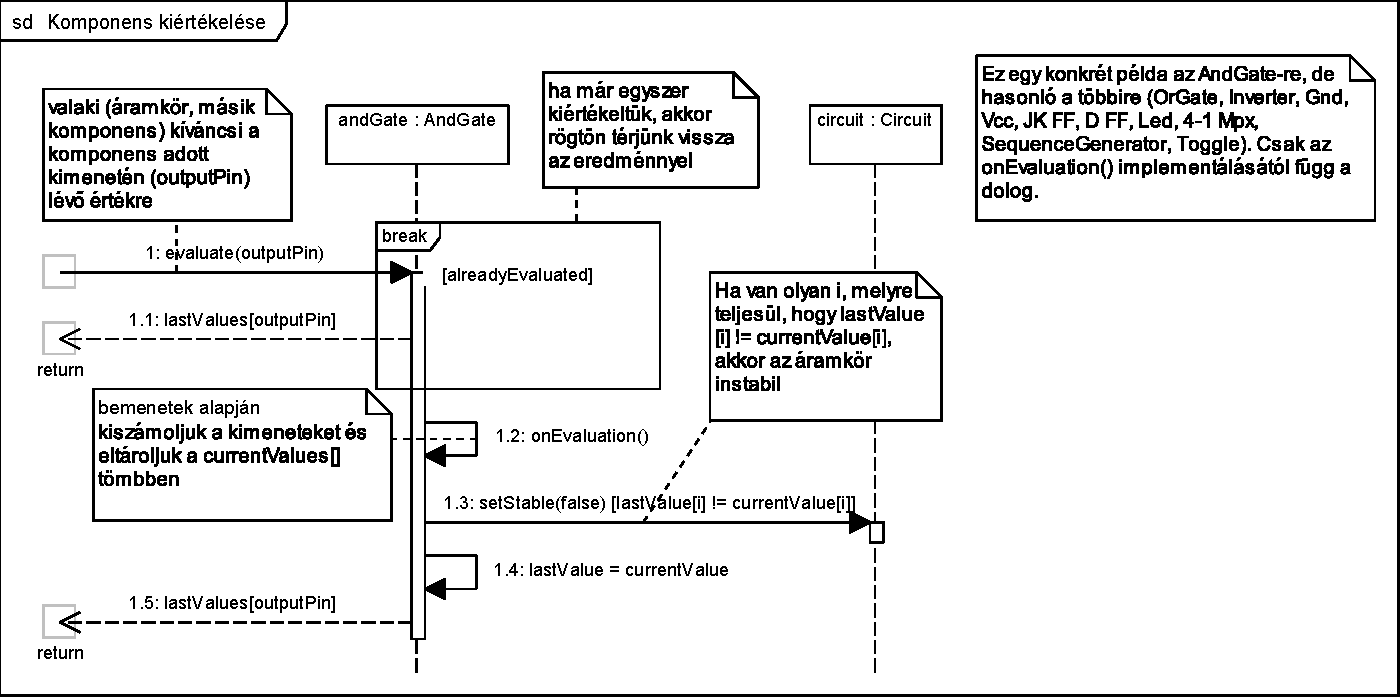
\includegraphics[angle = 90]{chapters/chapter03/seqdiagrams/sim_evaluate.pdf}
\caption{Komponens kiértékelése}
\label{fig:sim_evaluate}
\end{center}
\end{figure}

\begin{figure}[H]
\begin{center}
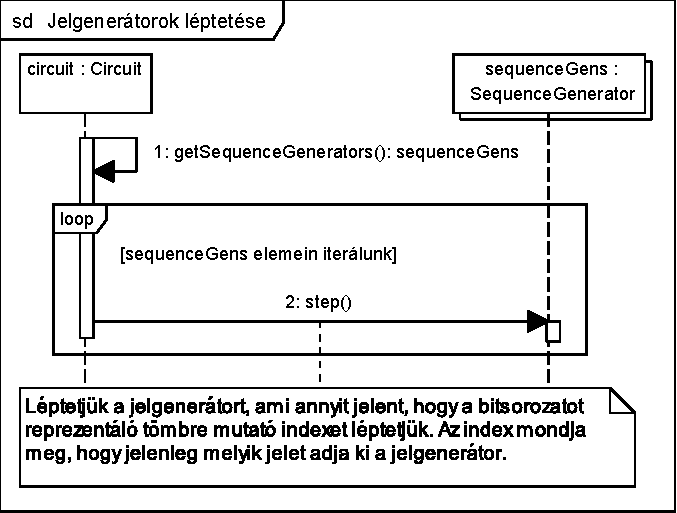
\includegraphics{chapters/chapter03/seqdiagrams/sim_stepGenerators.pdf}
\caption{Jelgenerátorok léptetése}
\label{fig:sim_stepGenerators}
\end{center}
\end{figure}

\begin{figure}[H]
\begin{center}
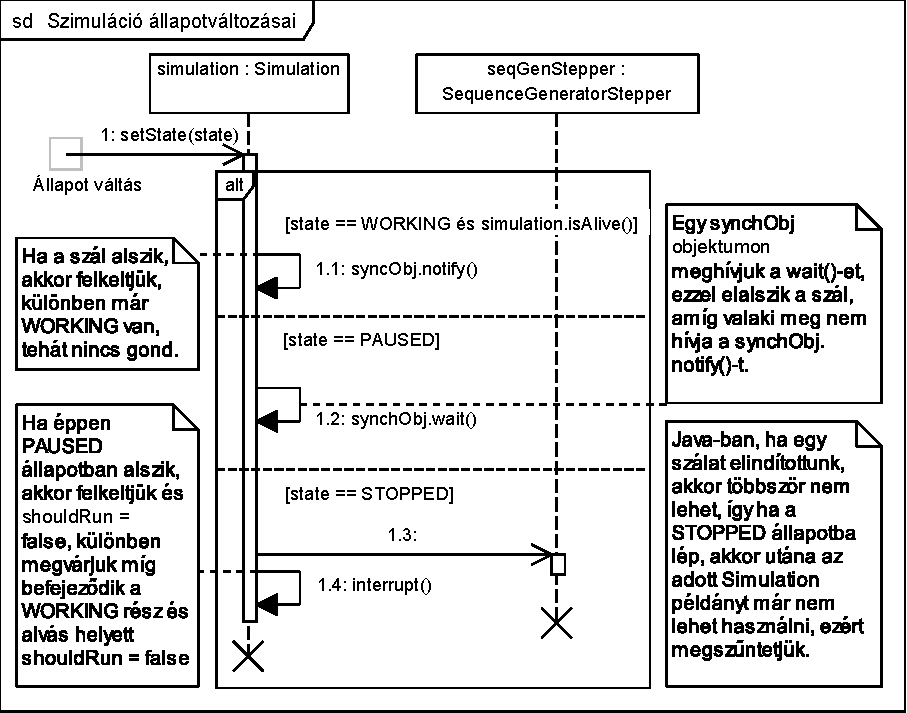
\includegraphics{chapters/chapter03/seqdiagrams/sim_allapotvaltozasai.pdf}
\caption{Szimuláció állapotváltozásai}
\label{fig:sim_allapotvaltozasai}
\end{center}
\end{figure}

\begin{figure}[H]
\begin{center}
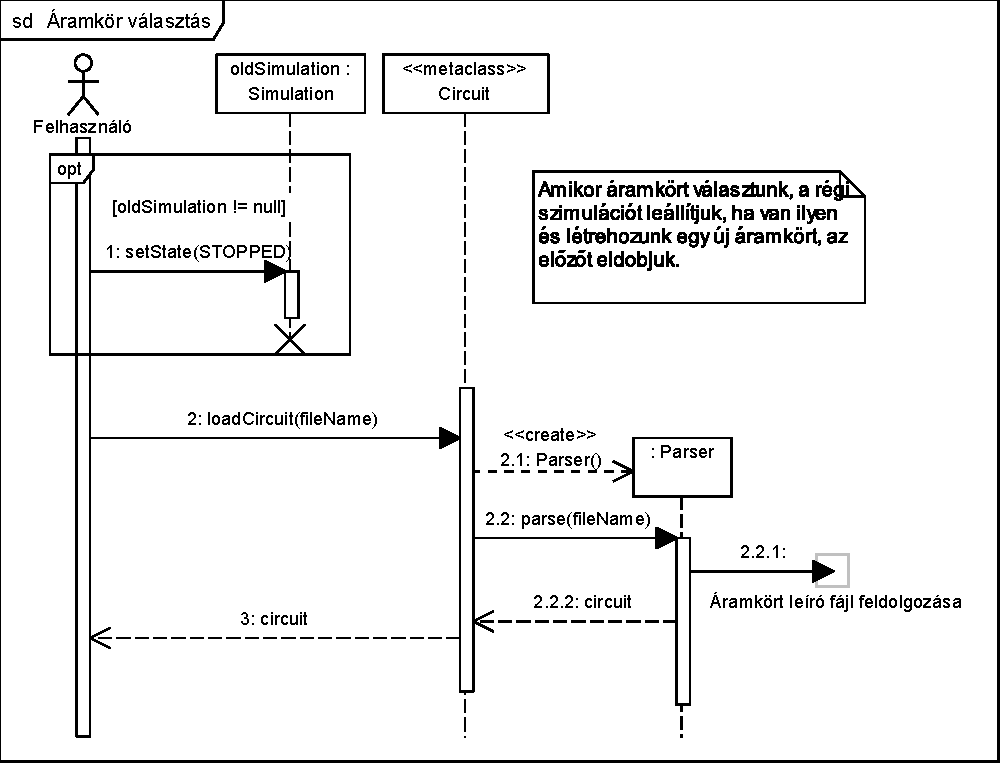
\includegraphics{chapters/chapter03/seqdiagrams/aramkor_valasztas.pdf}
\caption{Áramkör választás}
\label{fig:aramkor_valasztas}
\end{center}
\end{figure}

\begin{figure}[H]
\begin{center}
\includegraphics*[viewport = 0 581 500 990]{chapters/chapter03/seqdiagrams/aramkor_betoltese_fajlbol.pdf}
\caption{Áramkör betöltése fájlból 1. rész (vágva)}
\label{fig:aramkor_betoltese_fajlbol}
\end{center}
\end{figure}

\begin{figure}[H]
\begin{center}
\includegraphics*[viewport = 0 0 500 581]{chapters/chapter03/seqdiagrams/aramkor_betoltese_fajlbol.pdf}
\caption{Áramkör betöltése fájlból 2. rész}
\label{fig:aramkor_betoltese_fajlbol}
\end{center}
\end{figure}

\begin{figure}[H]
\begin{center}
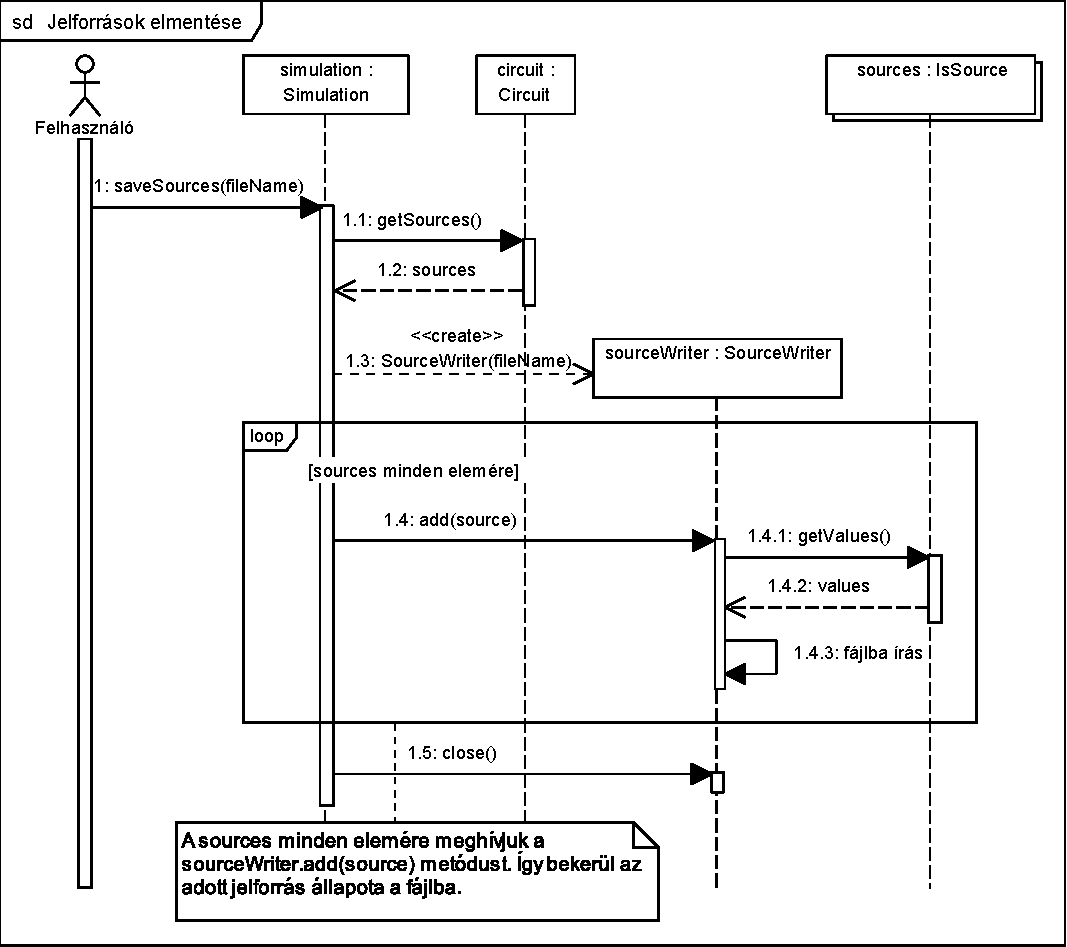
\includegraphics[width=17cm]{chapters/chapter03/seqdiagrams/jelforrasok_mentese.pdf}
\caption{Jelforrások mentése}
\label{fig:jelforrasok_mentese}
\end{center}
\end{figure}

\begin{figure}[H]
\begin{center}
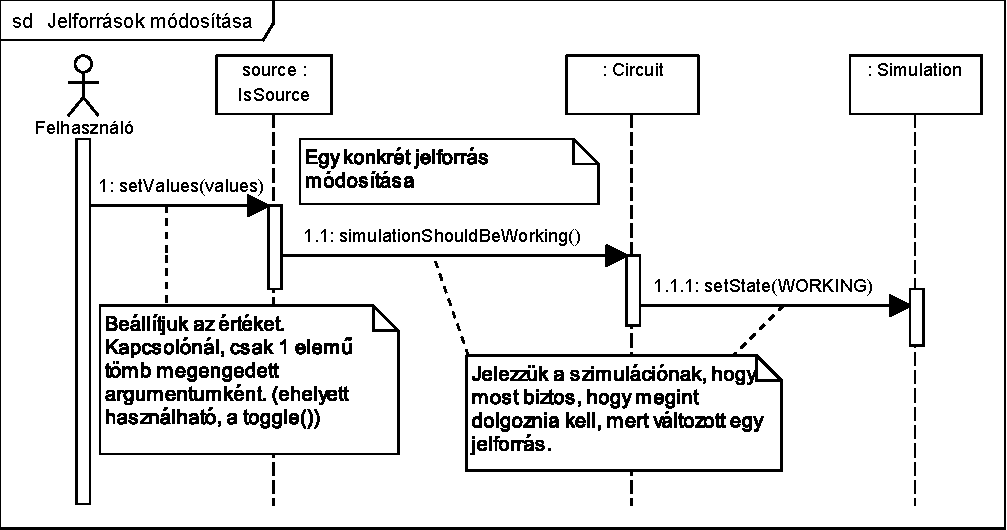
\includegraphics{chapters/chapter03/seqdiagrams/jelforrasok_modositasa.pdf}
\caption{Jelforrások módosítása}
\label{fig:jelforrasok_modositasa}
\end{center}
\end{figure}

\begin{figure}[H]
\begin{center}
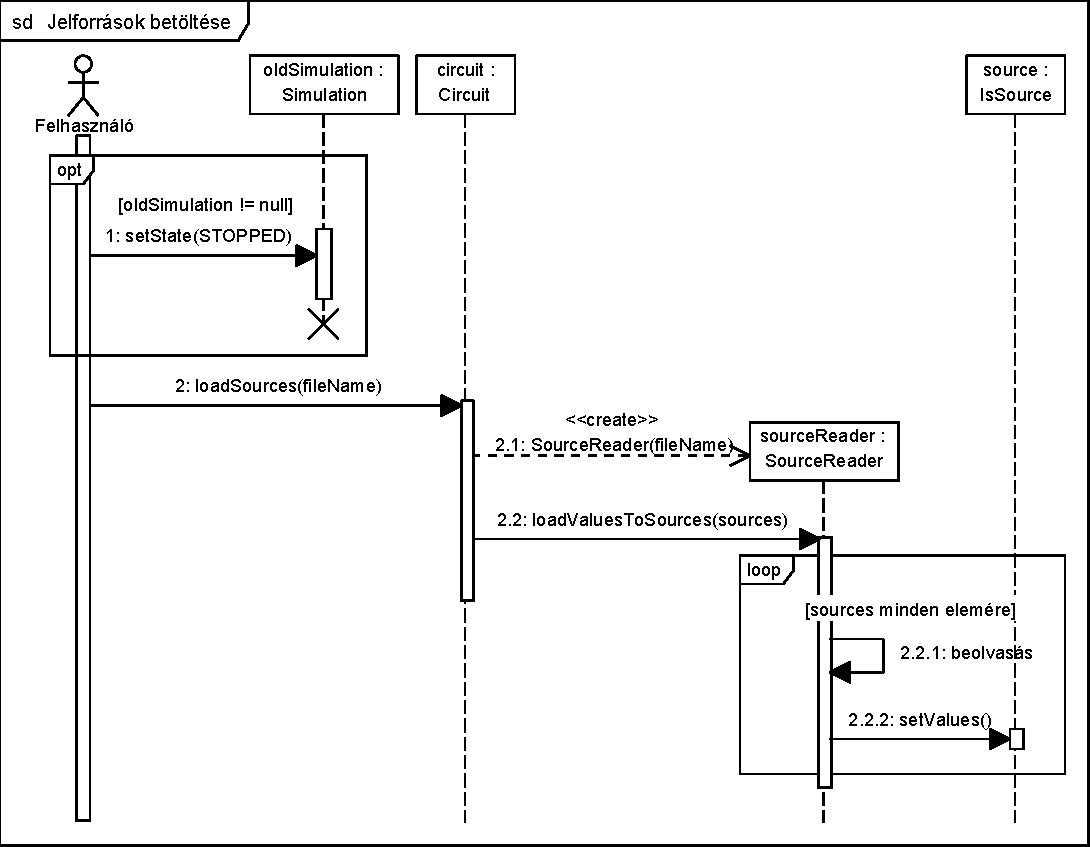
\includegraphics[angle=90]{chapters/chapter03/seqdiagrams/jelforrasok_betoltese.pdf}
\caption{Jelforrások betöltése}
\label{fig:jelforrasok_betoltese}
\end{center}
\end{figure}

\section{State-chartok}

\begin{figure}[h]
\begin{center}
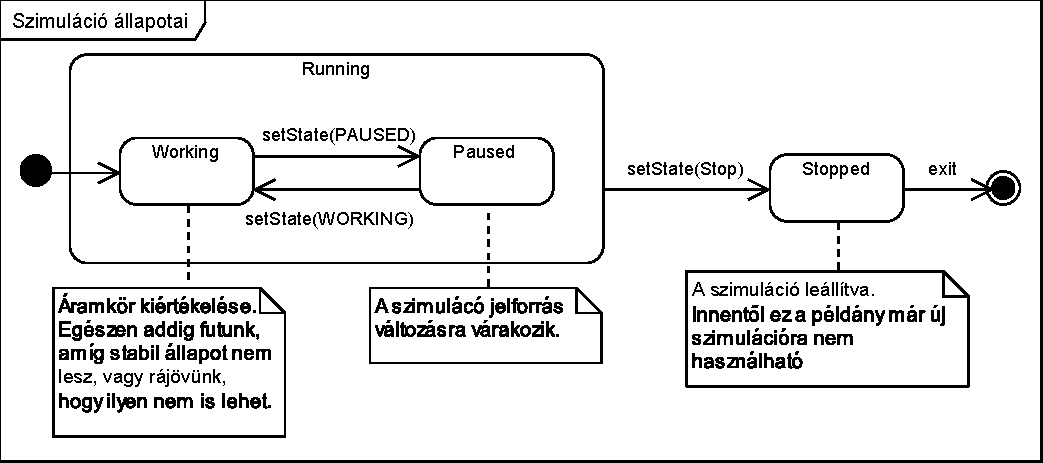
\includegraphics{chapters/chapter03/seqdiagrams/sim_states.pdf}
\caption{Szimuláció állapotai}
\label{fig:sim_states}
\end{center}
\end{figure}
